\section{Численная диагонализация решёточного\\ гамильтониана}
Как уже говорилось, краевые состояния не рассеиваются на потенциальном беспорядке, 
если нет объёмных или примесных состояний с той же энергией. 
Это можно увидеть непосредственно, 
диагонализуя решёточный гамильтониан. Из результатов численной диагонализации видно, что
краевые состояния огибают глубокое препятствие (см. рис.~\ref{fig:obstacle}).
\begin{figure}[h]
    \centering
    \begin{minipage}[t]{0.4\linewidth}
        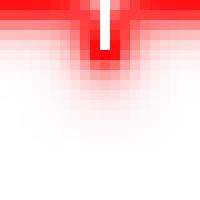
\includegraphics[width=0.9\linewidth]{obstacle_1.png}
    \end{minipage}
    \hfill
    \begin{minipage}[t]{0.4\linewidth}
        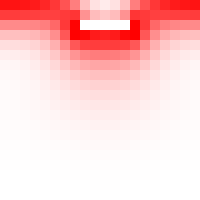
\includegraphics[width=0.9\linewidth]{obstacle_2.png}
    \end{minipage}
    \caption{
        Квадрат амплитуды волновой функции краевого состояния, огибающего препятствия. 
        Размер решётки --- $20\times20$, по горизонтальной оси наложены периодические
        граничные условия.
    }
    \label{fig:obstacle}
\end{figure}

Также краевые состояния <<выживают>> под действием даже довольно сильного потенциального
беспорядка
\begin{equation}
    \hat{V} = \sum_{m,n} V_{mn} (a_{mn}^\dagger a_{mn} + b_{mn}^\dagger b_{mn}),
\end{equation}
где $V_{mn}$ равномерно распределены по отрезку $[-\frac{W}{2}, \frac{W}{2}]$, см.
рис.~\ref{fig:disordered_stripe}.

\begin{figure}[h]
    \centering
    \begin{minipage}[h]{0.4\linewidth}
        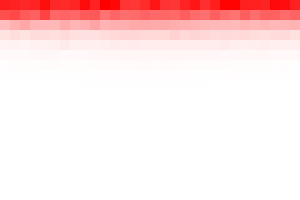
\includegraphics[width=1.\linewidth]{dis_edge_state_1.png}
        \caption{
            Волновая функция краевого состояния с беспорядком.
            Параметры модели: $\xi, m, t = -0.2, 1, 0.4$, сила беспорядка --- $0.5$.
            }
    \end{minipage}
    \hfill
    \begin{minipage}[h]{0.4\linewidth}
        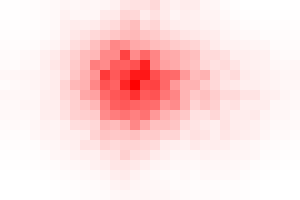
\includegraphics[width=1.\linewidth]{dis_bulk_state.png}
        \caption{
            Волновая функция объемного состояния с беспорядком для тех же параметров.
            }
    \end{minipage}
    \label{fig:disordered_stripe}
\end{figure}

Магнитный беспорядок, как нарушающий $T$--симметрию, приводит к рассеянию состояний
с двумя компонентами спина друг в друга. Это приводит к локализации краевых состояний,
что продемонстрировано на рис.~\ref{fig:magnetic_disorder}.  Магнитный беспорядок 
в симуляции имел вид
\begin{equation}
    \hat{V}_{\mathrm{mgn}} = \sum_{mn} J \hat{\sigma}_{mn} S_{mn},
\end{equation}
$\hat{\sigma}$ --- оператор спина на узле, $S_{mn}$ --- случайный вектор на единичной сфере.
\begin{figure}[h]
    \centering
    \begin{minipage}[h]{0.9\linewidth}
        \centering
        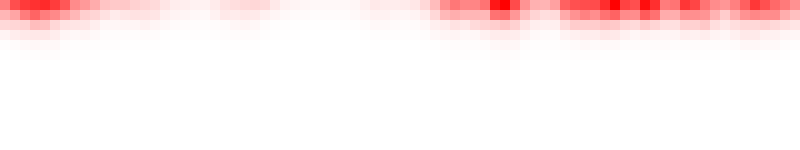
\includegraphics[width=0.7\linewidth]{mgn_edge_st_1.png}
    \end{minipage}
    \vfill
    \begin{minipage}[h]{0.9\linewidth}
        \centering
        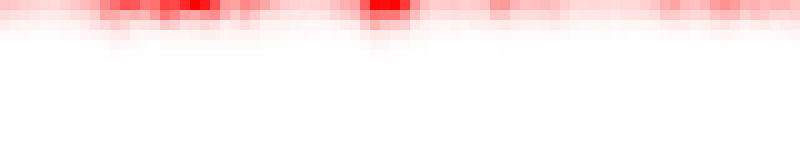
\includegraphics[width=0.7\linewidth]{mgn_edge_st_2.png}
    \end{minipage}
    \vfill
    \begin{minipage}[h]{0.9\linewidth}
        \centering
        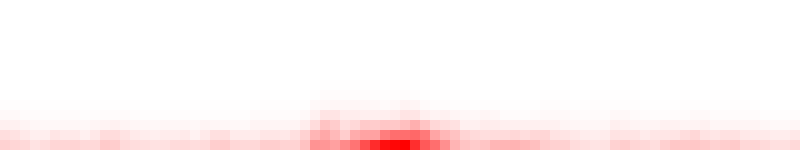
\includegraphics[width=0.7\linewidth]{mgn_edge_st_3.png}
    \end{minipage}
    \caption{
        Волновые функции краевых состояний с магнитным беспорядком 
        для тех же параметров.
        }
    \label{fig:magnetic_disorder}
\end{figure}

Также мы диагонализовали гамильтониан для случая, когда энергии примесных состояний
лежат в середине щели (см. рис.~\ref{fig:impurity_numeric_levels}). Для этого нужно
специальным образом подобрать силу возмущения.

\begin{figure}[h]
    \centering
    \begin{minipage}[h]{0.9\linewidth}
        \centering
        
\includegraphics[width=0.7\linewidth]{fig2.png}
    \end{minipage}
    \vfill
    \begin{minipage}[h]{0.9\linewidth}
        \centering
        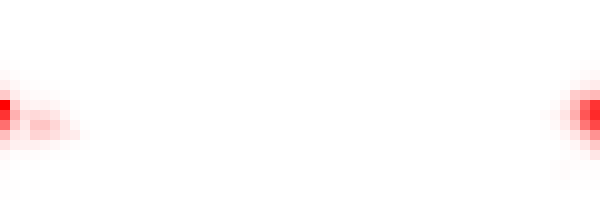
\includegraphics[width=0.7\linewidth]{fig3.png}
    \end{minipage}
    \vfill
    \begin{minipage}[h]{0.9\linewidth}
        \centering
        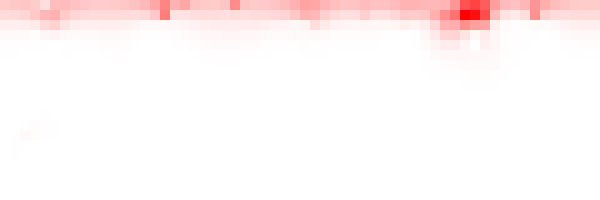
\includegraphics[width=0.7\linewidth]{fig5.png}
    \end{minipage}
    \caption{
        Волновые функции краевых состояний c примесями внутри щели      
    }

    \label{fig:magnetic_disorder}
\end{figure}
